% Ваш основной текст
\clearpage
\phantomsection% ensures hyperref works properly
\addcontentsline{toc}{section}{\hspace*{-1em}Приложение В (Обязательное) Python описание обучения сети}\par

\normalsize
\begin{center}
  \textbf{ПРИЛОЖЕНИЕ В} \\
  \textbf{(Обязательное)} \\
  \textbf{Python описание обучения сети}
\end{center}

Python описание обучения сети:

\lstinputlisting[language=python]{C/learn.py}

% Установка размера страницы A3 в альбомной ориентации
% \pdfpagewidth=420mm
% \pdfpageheight=297mm

% \thispagestyle{empty} % Убрать номер страницы

% % Вставка листа A3
% 
\includepdf[pages=-, pagecommand={}, fitpaper, offset=0 0]{STRUCT.pdf}

% Восстановление размера страницы A4
% \pdfpagewidth=210mm
% \pdfpageheight=297mm
% 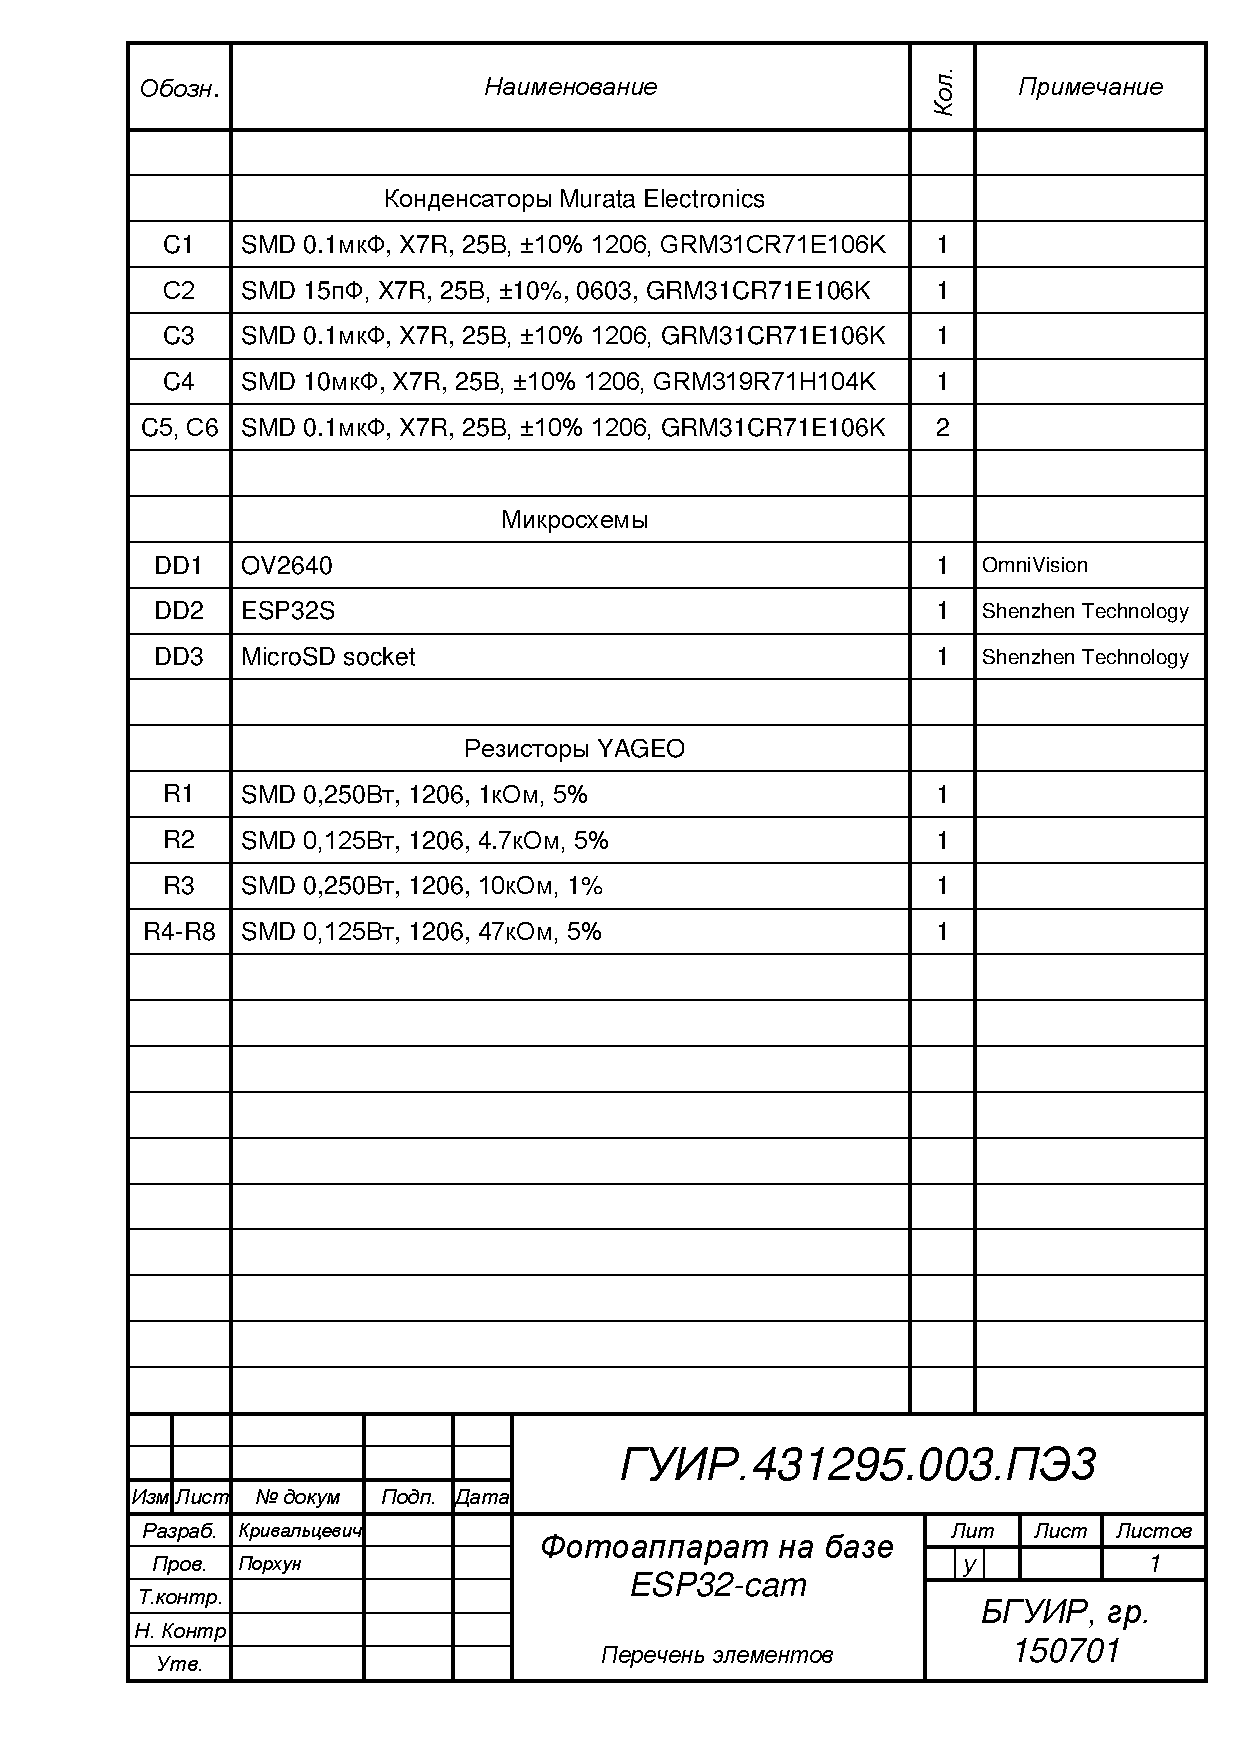
\includepdf[pages=-, pagecommand={}, fitpaper, offset=0 0]{perechen.pdf}
% \clearpage
